\documentclass{article}
\usepackage[utf8]{inputenc}
\usepackage[ngerman]{babel}
\usepackage[T1]{fontenc}
\usepackage{lmodern}
\usepackage{graphicx}
\usepackage[locale=DE]{siunitx}
\usepackage{float}
\usepackage[nottoc,numbib]{tocbibind}
\newcommand{\RM}[1]{\MakeUppercase{\romannumeral #1}}


\usepackage{longtable}

\usepackage{bibgerm}

\usepackage{footnpag}

\usepackage{ifthen}

\usepackage{graphicx}

\usepackage{here}

\usepackage{amsmath}

\usepackage{amsxtra}

\usepackage{amsfonts}

\usepackage{amssymb}

\usepackage{url}

%FÃŒr Testzwecke aktivieren, zeigt labels und refs im Text an.

%\usepackage{showkeys}

% Abstand zwischen zwei AbsÀtzen nach DIN (1,5 Zeilen)

\setlength{\parskip}{1.5ex plus0.5ex minus0.5ex}

% EinrÃŒckung am Anfang eines neuen Absatzes nach DIN (keine)

\setlength{\parindent}{0pt}

% RÀnder definieren

\setlength{\oddsidemargin}{0.3cm}

\setlength{\textwidth}{15.6cm}

% bessere Bildunterschriften

\usepackage[center]{caption2}

% Problemlösungen beim Umgang mit Gleitumgebungen

\usepackage{float}

% Nummeriert bis zur Strukturstufe 3 (also <section>, <subsection> und <subsubsection>)

\setcounter{secnumdepth}{3}

% FÃŒhrt das Inhaltsverzeichnis bis zur Strukturstufe 3

\setcounter{tocdepth}{3}

\usepackage{exscale}





% fÌhrt mit \vv zu lÀngenangepassten vektorpfeilen

\usepackage{esvect}

%Ergibt eine nummerierte AufzÀhlung bei enumerate

%\begin{compactenum}[(i)] fÃŒhrt zu (i), (ii), (iii), (iv), ...

%\begin{compactenum}[(I)] fÃŒhrt zu (I), (II), (III), (IV), ...

%\begin{compactenum}[a)] fÃŒhrt zu a), b), c), d), ...

\usepackage{paralist}


\newenvironment{dsm} {\begin{displaymath}} {\end{displaymath}}

\newenvironment{vars} {\begin{center}\scriptsize} {\normalsize \end{center}}

\newcommand {\en} {\varepsilon_0} % Epsilon-Null aus der Elektrodynamik

\newcommand {\lap} {\; \mathbf{\Delta}} % Laplace-Operator

\newcommand {\R} { \mathbb{R} } % Menge der reellen Zahlen

\newcommand {\e} { \ \mathbf{e} } % Eulersche Zahl

\renewcommand {\i} { \mathbf{i} } % komplexe Zahl i

\newcommand {\N} { \mathbb{N} } % Menge der nat. Zahlen

\newcommand {\C} { \mathbb{C} } % Menge der kompl. Zahlen

\newcommand {\Z} { \mathbb{Z} } % Menge der kompl. Zahlen

\newcommand {\limi}[1]{\lim_{#1 \rightarrow \infty}} % Limes unendlich

\newcommand {\sumi}[1]{\sum_{#1=0}^\infty}

\newcommand {\rot} {\; \mathrm{rot} \,} % Rotation

\newcommand {\grad} {\; \mathrm{grad} \,} % Gradient

\newcommand {\dive} {\; \mathrm{div} \,} % Divergenz

\newcommand {\dx} {\; \mathrm{d} } % Differential d

\newcommand {\cotanh} {\; \mathrm{cotanh} \,} %Cotangenshyperbolicus

\newcommand {\asinh} {\; \mathrm{areasinh} \,} %Area-Sinus-Hyp.

\newcommand {\acosh} {\; \mathrm{areacosh} \,} %Area-Cosinus-H.

\newcommand {\atanh} {\; \mathrm{areatanh} \,} %Area Tangens-H.

\newcommand {\acoth} {\; \mathrm{areacoth} \,} % Area-cotangens

\newcommand {\Sp} {\; \mathrm{Sp} \,}

\newcommand {\mbe} {\stackrel{\text{!}}{=}} %Must Be Equal

\newcommand{\qed} { \hfll $\square$\\}

\renewcommand{\i} {\imath}

\newcommand{\ham}{\mathcal{H}}

\newcommand{\lag}{\mathcal{L}}

\def\captionsngerman{\def\figurename{\textbf{Abb.}}}

\renewcommand{\dagger}{**}

\renewcommand{\contentsname}{Inhaltsverzeichnis}

\renewcommand{\figurename}{Abbildung}

\renewcommand{\tablename}{Tabelle}

\usepackage{url}
\begin{document}
	
	
	
	\scriptsize \normalsize
\title{Rutherford-Streuung \\ Versuch 16}



\author{Polina Stecher\\ {polina.stecher@tu-dortmund.de} \and Ramona Gabriela Kallo \\{ramonagabriela.kallo@yahoo.de} } %{polina.stecher@tu-dortmund.de  sonya.djuffouo@tu-dortmund.de} 
\date{Durchgeführt am 12. Dezember 2018\\Korrektur}
\maketitle
\newpage

\tableofcontents
\thispagestyle{empty}
	\newpage 
	
\section{Zielsetzung und Motivation}
\label{sec:ZielsetzungundMotivation}
Das Ziel dieses Versuchs ist es die Streuung von $\alpha$-Teilchen an einer Goldfolie zu bestimmen. Dafür wird der differentielle Wirkungsquerschnitt der Streuung an einer dünnen Goldfolie und die Abhängigkeit der Kernladungszahl $Z$ des Targetmaterials untersucht.
Am Ende soll mittels einer Energieverlustmessung der $\alpha$-Teilchen auch die Foliendicke bestimmt werden.

\section{Theorie}
\label{sec:Theorie}
Bei der Wechselwirkung von positiv geladenen $\alpha$-Teilchen durch Materie kann es zu zwei Effekten kommen. Zum einen können die $\alpha$-Teilchen mit dem Kern wechselwirken und werden dabei gestreut und zum anderen können sie mit den negativ geladenen Hüllenelektronen wechselwirken. Dabei verlieren sie Energie und werden langsamer. 

\subsection{Bethe-Bloch-Gleichung}
Bei der Wechselwirkung der $\alpha$-Teilchen mit dem Hüllenelektronen kommt es durch Ionisation oder Anregung der Atome oder Moleküle der durchstrahlten Materie zur Energieabgabe. Der Energieverlust pro Wegstrecke eines $\alpha$-Teilchens beim Durchqueren von Materie wird mittels Bethe-Bloch-Gleichung beschrieben:
\begin{equation}
\label{eq:bethebloch}
-\frac{dE}{dx} = - \frac{4 \pi e^4 z^2 N Z}{m_0 v^2 (4\pi\epsilon_0)^2}\text{ln}\left(\frac{2 m_0 v^2}{I}\right),
\end{equation}
wobei $N$ die Atomdichte, $m_0$ die Ruhemasse eines Elektrons, $z$ die Ladungszahl des $\alpha$-Teilchens, $Z$ die Kernladungszahl des Targetmaterials, $I$ die mittlere Ionisationsenergie, $v$ die Geschwindigkeit des Ions und $E$ die Energie des Teilchens sind.

\subsection{Rutherford Streuformel}
Bei der Streuung der $\alpha$-Teilchen am Kern, erfahren sie durch die Coulombabstoßung eine Richtungsänderung um den Streuwinkel $\Theta$. Dieser Typ von Wechselwirkung lässt sich mit der Rutherfordschen Streuformel beschreiben:
\begin{equation}
\frac{d\sigma}{d\Omega}(\Theta) = \frac{1}{4 \pi \epsilon_0} \left(\frac{z Z e^2}{4 E_\alpha}\right)^2 \frac{1}{\text{sin}^4 \frac{\Theta}{2}},
\end{equation}
wobei $E_\alpha$ die mittlere kinetische Energie der $\alpha$-Teilchen und $\Theta$ den Winkel zwischen einfallendem und gestreutem $\alpha$-Teilchen beschreibt. Der differentielle Wirkungsquerschnitt $\frac{d\sigma}{d\Omega}$ gibt mit welcher Wahrscheinlichkeit für ein bestimmtes Teilchen an, in dem Raumwinkel $d\Omega$ gestreut zu werden.


\section{Versuchsaufbau und Durchführung}
\label{sec:Durchführung}
Der Versuchsaufbau wird schematisch in der Abbildung \ref{fig:versuchsaufbau} dargestellt. Da die $\alpha$-Teilchen eine geringe Reichweite($\SI{10}{\centi\meter}$) in Luft haben, wird der Versuch in Vakuum durchgeführt, um die Wechselwirkung mit den Stoßpartnern(Luftmolekülen), an die die $\alpha$-Teilchen ihre kinetische Energie sukzessive abgeben, zu verhindern. Als Quelle dient ein $^{241}$Am-Präparat, das mit einer Halbwertszeit von $420$ Jahren zu Neptunium zerfällt. Die $\alpha$-Teilchen haben eine Energie von $\SI{132}{\frac{\mega\electronvolt}{\meter}}$.
\begin{figure}[h!]
	\centering
	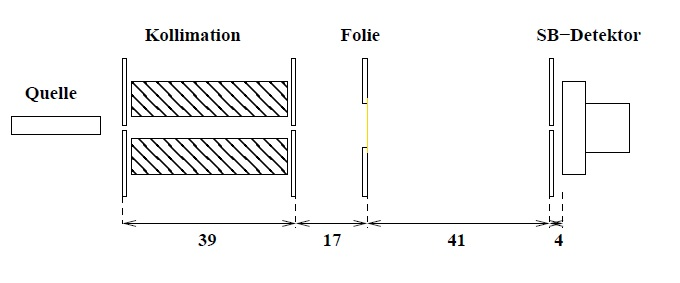
\includegraphics[width=0.9\linewidth]{Versuchsaufbau.jpg}
	\caption{Zu sehen ist der schematische Aufbau des Versuches. Der Abstand zwischen den einzelnen Bauteilen der Messapparatur werden in Millimeter angegeben $^{[1]}$}

\end{figure}
Die Strahlen aus der Quelle werden mithilfe von zwei $\SI{2}{\milli\meter}$ Schlitzblenden kollimiert und werden durch die Blenden gebündelt. Der Strahl trifft anschließend senkrecht auf die Goldfolie, wo dann die Wechselwirkung mit Materie stattfindet. Die gestreuten $\alpha$-Teilchen werden in Abhängigkeit des Streuwinkels von einem Halbleiter-Detektor, also einem Surface-Barrier-Detektor detektiert. Bei diesem Detektor handelt es sich um eine in Sperrrichtung betriebene Diode, in der die einfallenden $\alpha$-Teilchen Elektronen-Loch-Paare erzeugen, die zur Elektrode beschleunigt werden. Der aufgenommene Impuls wird durch einen Multiplier verstärkt und ist proportional zur Energie des Teilchens. Außerdem sind ein Oszilloskop für die Energieverlustmessung und ein Zähler für die Streuquerschnittmessung vorhanden.

Zuerst wird die Streukammer mit einer Vakuumpumpe evakuiert. Die Sperrspannung des Surface-Barrier-Detektors wird auf $\SI{12}{\volt}$ eingestellt. Der Detektor wird justiert, um einen geraden Durchtritt  der $\alpha$-Teilchen zu gewährleisten. Anschließend wird eine Energieverlustmessung der Foliendicke durchgeführt. Dazu wird die Pulshöhe der Detektorpulse in Abhängigkeit von verschiedenen Kammerdrücken gemessen. Dieser Messvorgang wird zunächst mit und anschließend ohne eingesetzter Folie durchgeführt. Mithilfe von einem Feindrosselventil wird der Kammerdruck langsam erhöht. Zur Ermittlung der mittleren Pulshöhe wird das Oszilloskop in das Programm "Nachleuchten" gestellt, an dem dann die Pulshöhen abgelesen werden können. Im weiteren Verlauf des Versuches soll der differentielle Streuquerschnitt für eine $\SI{2}{\micro\meter}$ dünne Goldfolie untersucht werden. Hierfür wird die Zählrate in Abhängigkeit des Streuwinkels gemessen. Für diese Messung werden verschiedene Winkel eingestellt. Da der der $\alpha$-Zerfall poissonverteilt ist, wird versucht den Fehler möglichst klein zu halten. Der statistische Fehler dieser Messung für die Zählrate beträgt $\sqrt{I}$. Für die Messung der Mehrfachstreuung wird der Streuquerschnitt mithilfe von einer anderen Goldfolie mit einer Dicke von $\SI{4}{\micro\meter}$ bei einem festen Winkel von $15 ^\circ$ gemessen.



	
\section{Auswertung}


\subsection{Vorbereitungsaufgabe}
\subsubsection{Termschema des Americium-Präparates}
\begin{figure}[h!]
	\centering
	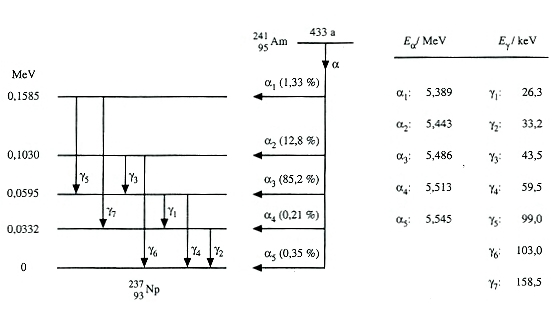
\includegraphics[width=0.9\linewidth]{6362cb7a8529daf05d8e0be425b50d10bacfe0c3}
	\caption{Zerfallsschema des Americium-Präparates $^{[2]}$}
	
\end{figure}
\subsubsection{Annahmen zur Herleitung der Bethe-Bloch-Gleichung und der Rutherfordschen Streuformel}
Für die Herleitung der Bethe-Bloch-Gleichung wird angenommen, dass das schwere Teilchen eine Ruhemasse $m_0$ besitzt, die deutlich größer ist als die Ruhemasse eines Elektrons ($m_0 \gg m_e$). Eine Ablenkung bei der Wechselwirkung kommt also in diesem Fall nicht in Frage. Es wird vor allem noch angenommen, dass das Hüllenelektron sich vor der Wechselwirkung in Ruhe befindet und dieses frei ist.

Für die Rutherfordschen Streuformel wird angenommen, dass das Atom einen positiv geladenen Kern hat und dass sich um den Kern die negative Elementarladungen, Elektronen, mit verschwindend kleiner Masse befinden. Während der Streuung wird der Kern als ruhend angenommen, weil dieser eine höhere Masse als das $\alpha$-Teilchen besitzt. Als letztes wird noch angenommen, dass keine Mehrfachstreuung auftritt.

\subsubsection{Bestimmung des Bremsvermögens in Luft für die Alpha-Teilchen}
Trockene Luft besteht hauptsächlich aus rund $\SI{78,08}{\percent}$ Stickstoff und $\SI{20,95}{\percent}$ Sauerstoff. Mithilfe der Ionisationsenergien der beiden Stoffe sowie Ordnungs- und Massenzahlen wird mittels eine Mittelwertrechnung für Luft die folgenden Werte 
(s.Tabelle 1) berechnet:

\begin{table}[htpb]
	\centering
	\caption{Die Bestandteile aus Luft und die Mittelwertrechnung $^{[3,4]}$} 
	\begin{tabular}{c|c|c|c}
		
		Stoff	&	Ordnungszahl / Z &	Massenzahl / A &  Ionisationsenergie $/ \si{\electronvolt}$\\
		\hline
		Sauerstoff & 	8 & 16 & 13,61 \\
		Stickstoff &	7 & 14 & 14,52 \\
		Luft & 	7,2 & 14,41 & 14,33 \\
		
	\end{tabular}
\end{table}

Unter den Standardbedingungen (T = $\SI{298,15}{\kelvin}$)[3] beträgt die Luftdichte den folgenden Wert:
\begin{equation}
\rho = \SI{1,184}{\kilogram\per\cubic\meter}
\end{equation}
Damit kann das Bremsvermögen von $\alpha$-Teilchen in Luft berechnet werden und beträgt:
\begin{equation*}
-\frac{dE}{dx} = \SI{132}{\frac{\mega\electronvolt}{\meter}}
\end{equation*}
Mit dem allgemeinen Gasgesetz kann anschließend der Luftdruck ermittelt werden:
\begin{equation}
p = \frac{\rho R T}{M}
\end{equation}
wobei $R$ die allgemeine Gaskonstante, $T$ die Temperatur unter den Standardbedingungen $\SI{298,15}{\kelvin}$ und $M$ die Molare Masse sind. Mit der Gleichung \ref{eq:bethebloch} wird für eine Wegstrecke von $\SI{100}{\milli\meter}$ ein Luftdruck von $\SI{12,19}{\pascal}$ berechnet.
\subsection{Beobachtung  der vorverstärkten Pulse am Oszilloskop}

\begin{figure}[H]
	\centering
	\includegraphics[height=8cm,width=12cm]{F0014TEK.jpg}
	\caption{ Verstärktes Signal, Aufnahme des Oszilloskops}
	\label{fig: abb. 1}
\end{figure} 
	
	\begin{figure}[H]
	
	\centering
	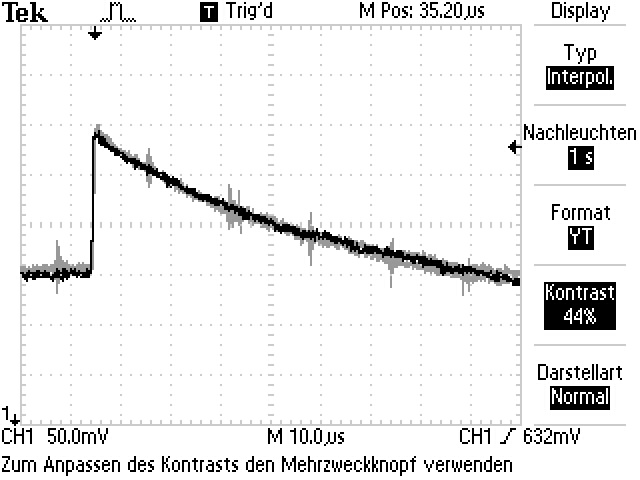
\includegraphics[height=8cm,width=12cm]{F0017TEK.jpg}
	\caption{ Nicht verstärktes Signal, Aufnahme des Oszilloskops}
	\label{fig: abb. 1}
	
	
\end{figure} 

Bei der Betrachtung der beiden Pulse in Abbildung (2) und (3) ist zu erkennen, dass die unverstärkte Aufnahme deutlich mehr Störungen aufweist. Außerdem ist der Kurvenverlauf der beiden Abbildung unterschiedlich. Bei dem verstärkten Puls handelt es sich um einen gauß'schen Verlauf, während der nicht verstärkte Puls einen senkrechten Anstieg und einen exponentialen Abstieg besitzt. Die Anstiegszeiten bei denen beide Pulse ihr Maximum erreichen, betragen: 
\begin{align*}
t_{verstärkt}=1 \text{ $\mu$s} \\
t_{unverstärkt}= 0,2\text{ $\mu$s} 
\end{align*}
Die Pulshöhen betragen:

\begin{align*}
I_{verstärkt}=\SI{4,20}{V}\\
I_{unverstärkt}=\SI{0,14}{V}
\end{align*}

\subsection{Aktivitätsbestimmung der Probe}

Zur Bestimmung der Aktivität wurden folgende Werte gemessen


\begin{table}[H] 
	\centering
	\begin{tabular}{c|c|c|c}
		
		Zählrate n  & Fehler der Zählrate $\sqrt{n}$ & $n/t \, / s^{-1}$& t / s \\ 
		\hline 
		5033&70,94 & 16,78 $ \pm$ 0,24&300\\

		
	\end{tabular} 
	\caption{Nullmessung } 
\end{table} 
Mit dem Raumwinkel 
\begin{align}
d\Omega= 4 \arctan\left(\frac{x}{2L}\right) \arctan\left(\frac{y}{2L} \right) =0,0098
\end{align}
wobei $L=\SI{4,5}{cm}$ der Abstand zwischen der Folie und dem Detektor ist und der durch die Blenden begrenzte Fläche beträgt $x=\SI{2}{mm}$ und $y=\SI{10}{mm}$,
wird die experimentelle Aktivität mit Hilfe der Formel 
\begin{align}
A_{exp}=\dfrac{4\pi}{d\Omega}=(21,52 \pm 0,31) \, \text{kBq}
\end{align}
bestimmt.  Das Zerfallsgesetz lautet:
\begin{align}
A(t)=A(0)\cdot e^{-\lambda t}
\end{align}
Die Anfangsaktivität beträgt $A(0)=330 \text{kBq}^{[1]}$ und die Zerfallskonstante $\lambda= \dfrac{ln(2)}{T_{1/2}}=5,09 \cdot 10^{-11} \text{s$^{-1}$}$. Mit diesen Werten ergibt sich für die theoretische Aktivität am Versuchstag (12.12.2018):
\begin{align*}
A_{theo}=317\, \text{kBq}
\end{align*}



\subsection{Bestimmung der Foliendicke }

Zur Bestimmung der Foliendicke wurde eine Energieverlustmessung durchgeführt.
Die Messwerte sind in Tabelle 3 und 4 aufgelistet. 
\begin{table}[H] 
	\centering
	\begin{tabular}{c|c|c}
		
		Druck  / mbar& Pulshöhe / V& Fehler / V \\ 
		\hline 
		0,032& 4,08& 1,1\\
		11,0&3,88 & 1,0\\
		32,9& 3,44 &1,0\\
		48,0&3,35& 1,0 \\
		73,9&3,12& 0,9\\
		92,6& 2,88& 1,0\\
		103,9&2,60&0,8\\
		122,7&2,48& 0,8\\
		146,8& 2,04& 0,9\\
		189,9 & 1,40&1,0\\
		200,7&1,32&1,0\\
		225,2&1,20&0,9\\
		250,0& 0,68&0,8\\
		266,4&0,44&0,8\\
		282,2&0,20&0,8\\
		
		
	\end{tabular} 
	\caption{Messwerte für die Energieverlustmessung ohne Folie } 
\end{table}  

\begin{table}[H] 
	\centering
	\begin{tabular}{c|c|c}
		
		Druck / mbar& Pulshöhe  / V & Fehler / V\\ 
		\hline 
		0,20  & 2,84& 1,1\\ 
		
		10,9 & 2,64 &1,0\\ 
		
		28,0 &2,56 & 1,0\\ 
		
		35,8 & 2,40&0,9\\ 
		
		51,1 & 2,29 &0,9\\ 
		
		70,9 & 2,08&1,0 \\ 
		
		89,3 &  1,68 &0,8\\ 
		
		99,9 & 1,60 &0,9\\ 
		
		109,4 & 1,44 &0,9\\ 
		
		137,3 & 1,04 &1,0\\ 
		
		152,5 & 0,97& 1,0\\
		
		168,8 & 0,88&0,9\\
		
		178,3& 0,86&0,8\\
		
		190,7 & 0,52&0,9\\
		
		202,2& 0,2 &0,9\\
		
	\end{tabular} 
	\caption{Messwerte für die Energieverlustmessung mit Folie } 
\end{table} 

Anschließend wird die Pulshöhe gegen den Druck aufgetragen. 

	\begin{figure}[H]
	
	\centering
	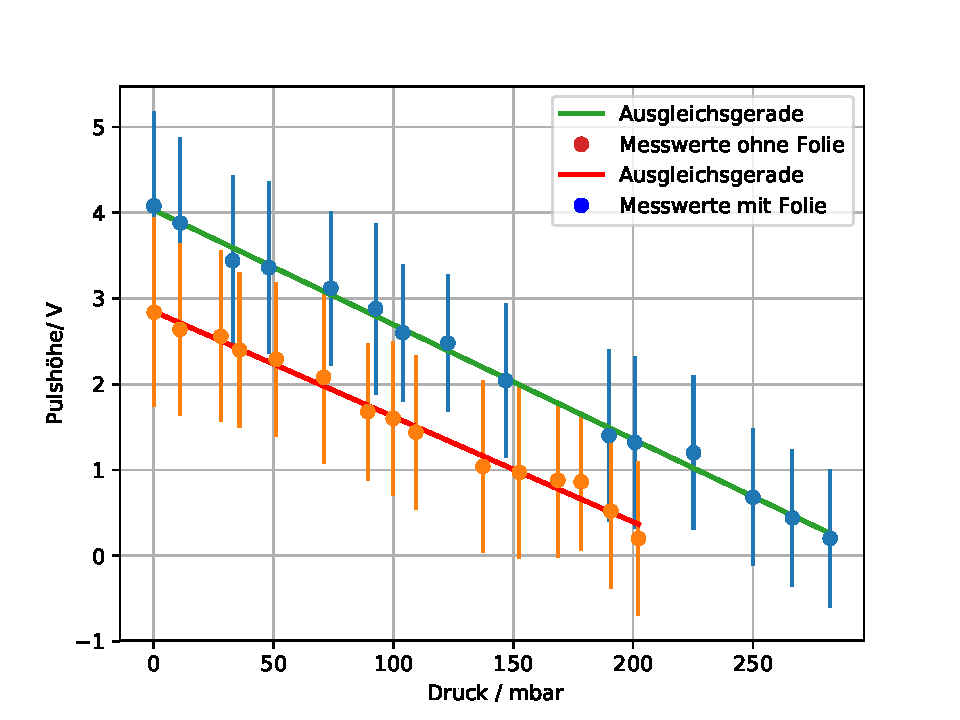
\includegraphics[height=8cm,width=12cm]{foliendicke.pdf}
	\caption{ Energieverlustmessung mit und ohne Folie}
	\label{fig: abb. 1}
	
	
\end{figure} 

Mit Hilfe der linearen Ausgleichsgerade der Form $f(x)=ax+b$ werden folgende Werte für die Parameter $a$ und $b$ erhalten:
\begin{align*}
a_{ohne}=( -13,4 \pm 0,24) \dfrac{\text{V}}{\text{bar}}\\
a_{mit}=(-12,3\pm 0,40)\dfrac{\text{V}}{\text{bar}}\\
b_{ohne}=(4,033\pm 0,04)\text{V}\\
b_{mit}=(2,849\pm 0,05)\text{V}
\end{align*}
Die Differenz dieser beiden Geraden entspricht dem Energieverlust durch die Folie.
Die Impulshöhendifferenz beträgt
\begin{align*}
\Delta I= b_{ohne}-b_{mit}=( 1,184\pm 0,062)\text{V}
\end{align*}
Die Energie eines $\alpha$-Teilchens beträgt $E_{\alpha}=5,27\cdot10^6 \text{eV}^{[2]}$.  Im Folgenden wird angenommen, dass das die Energie ist, die bei der Messung ohne Folie am Detektor detektiert wird. Unter dieser Annahme lässt sich der Energieverlust mit der Differenz der Impulshöhen berechnen zu:
\begin{align*}
	\Delta E= E_{\alpha} (1-\dfrac{b_{mit}}{b_{ohne}})= (1,55\pm 0,11) \cdot 10^6 \text{eV}
\end{align*}
Die Dicke $dx$ der Goldfolie lässt sich berechnen, indem die Bethe-Bloch-Gleichung (1) nach der Dicke $dx$ umgestellt wird und die materialspezifischen Parameter eingesetzt werden. Für die Masse des $\alpha$-Teilchens ergibt sich mit der Formel $m_{\alpha}=A\cdot u=6,64\cdot 10^{-27}\text{kg}^{[2]}$. A ist die elementarspezifische Massenzahl und u die atomare Masseneinheit. Für die Geschwindigkeit ergibt sich 
\begin{align*}
v_{\alpha}= \sqrt{\frac{2\cdot \bar{E}}{m_{\alpha}}} = 16,27\cdot10^6 \text{m/s}
\end{align*}
Die Alpha-Teilchen verlieren beim Durchfliegen von Materie Energie. Für die Berechnung der Geschwindigkeit wird die mittlere Energie $\bar{E}$ verwendet. 
\begin{align}
\bar{E}=\dfrac{1}{2}(E_{mit}+E_{ohne})=\dfrac{1}{2}\cdot \left(\dfrac{b_{mit}}{b_{ohne}}E_{ohne}+E_{ohne}\right)=\dfrac{1}{2}\cdot E_{ohne} \left(\dfrac{b_{mit}}{b_{ohne}}+1\right)=(4,5 \cdot 10^6) \text{eV}
\end{align}
Die Anzahl der Teilchen pro Volumeneinheit berechnet sich über 
\begin{align*}
N= \frac{\rho}{m}=5,91\cdot10^{28} \text{1/m$^3$}.
\end{align*}
Für die Dichte des Targetmaterials $\rho$ wird 19320 $\frac{\text{kg}}{\text{m}^3}^{[1]}$ eingesetzt. Die Masse wird wieder mittels des Produktes aus Massenzahl und atomarer Masseneinheit bestimmt. Die Masse von Gold mit A=197$^{[5]}$ beträgt $m_{Gold}=1.31 \cdot 10^{-25} $$^{[5]}$ kg. \\
Weiterhin beträgt die Ionisationsenergie von Gold $I=790\, \text{eV} \,^{[8]}$ und die Ordnungzahlen  z$_{\alpha}$=2 und Z$_{Gold}$=79. Somit ergibt sich für die Foliendicke $dx$ mit Hilfe der Formel (1):
\begin{align*}
dx=(3,45\pm 0,13) \mu\text{m}.
\end{align*}
\subsection{Bestimmung des differentiellen Streuquerschnittes}

Die zur Bestimmung des differentiellen Streuquerschnittes aufgenommen Werte sind in Tabelle 5 aufgelistet. 

\begin{table}[H] 
	\centering
	\begin{tabular}{c c c c|c c c c}
		
		Winkel /$^{\circ}$  & Zählrate n  & Zeit t /s   & n/t /s$^{-1}$ & Winkel  /$^{\circ}$  & Zählrate n  & Zeit t /s  & n/t /s$^{-1}$ \\ 
		\hline 
		0 & 2048 $\pm$ 45 & 300 & 6,83 $\pm$ 0,15& 10,6 & 729 $\pm$ 27& 300& 2,43$\pm$ 0,09\\ 
		
		1,5 & 1838 $\pm$ 43 & 300 & 6,13 $\pm$ 0,14  & 11,6 & 196 $\pm$ 14 & 300 & 0,65 $\pm$ 0,05\\ 
		
		2,1 & 1615 $\pm$ 40  & 300 & 5,38 $\pm$ 0,13& 12,8 & 92 $\pm$ 10 & 600 & 0,15 $\pm$ 0,02\\ 
		
		3,4 & 1197 $\pm$ 35 & 300 & 3,99 $\pm$ 0,11 & 14,1 & 81 $\pm$ 9 & 700  & 0,12 $\pm$ 0,01\\ 
		
		4,7 & 768  $\pm$ 28 & 300 & 2,56 $\pm$ 0,09 & 15,9 & 68 $\pm$ 8 & 800 & 0,08 $\pm$ 0,01 \\ 
		
		6,2& 462 $\pm$ 22 & 300 & 1,54 $\pm$ 0,07& 18,3& 106 $\pm$ 10 & 650 & 0,16 $\pm$ 0,01 \\ 
		
		7,4& 226 $\pm$ 15 & 300 & 0,75 $\pm$ 0,05& 20,2& 86  $\pm$ 9&600 & 0,14 $\pm$ 0,02\\ 
		
		9,2& 101 $\pm$ 10 & 300& 0,34 $\pm$ 0,03
		
		
		
	\end{tabular} 
	\caption{Messwerte für die Goldfolie} 
\end{table}
Der differentielle Wirkungsquerschnitt $\frac{d\sigma}{d\Omega}_{Mess}$ und der zugehörige Fehler $\Delta\frac{d\sigma}{d\Omega}_{Mess}$ werden mit folgenden Formeln bestimmt: 
\begin{align}
\frac{d\sigma}{d\Omega}_{Mess} (\theta)= \frac{n}{A \; N \; dx \; d\Omega}^{[9]}
\end{align}

\begin{align}
\Delta\frac{d\sigma}{d\Omega}_{Mess}= \sqrt{\left(\frac{\Delta n}{A\; N \; dx \; d\Omega}\right)^2+ \left(-\frac{\Delta A \;n}{A^2 \; N\; dx \; d\Omega}\right)^2}
\end{align}
Der Fehler $\Delta n$ wird mit der Formel $\Delta n=\dfrac{\sqrt{n}}{t}$ berechnet. A ist die Aktivität der Probe und beträgt $A=(16,7878\pm 0,23) \text{1/s}$. Der Raumwinkel ergibt sich über die Formel :
\begin{align}
d\Omega= 4 \arctan\left(\frac{x}{2L}\right) \arctan\left(\frac{y}{2L} \right) =0,0098
\end{align}
Die mit Formel (9) berechneten Wirkungsquerschnitte $\frac{d\sigma}{d\Omega}_{Mess}$ und die  über die Rutherfordschen Streuformel (2) ermittelten Werte $\frac{d\sigma}{d\Omega}_{Theo}$ sind in der nachfolgenden Tabelle aufgelistet.

 \begin{table}[H] 
	\centering
	\begin{tabular}{c c c |c c c }
		
		Winkel / $^{\circ}$  & $\frac{d\sigma}{d\Omega}_{Theo} / 10^{-22} \text{m$^2$}$ & $\frac{d\sigma}{d\Omega}_{Mess} /10^{-22} \text{m$^2$}$  & Winkel / $^{\circ}$  & $\frac{d\sigma}{d\Omega}_{Theo} / 10^{-22} \text{m$^2$}$  & $\frac{d\sigma}{d\Omega}_{Mess} / 10^{-22} \text{m$^2$}$   \\ 
		\hline 
		0 & - & 3.51 $\pm$ 0,071&  10,6& 0,01 & 1,25 $\pm$ 0,041\\ 
		
		1.5 & 36,6 & 3,15 $\pm$ 0,064& 11,6 & 0,01 & 0,34 $\pm$ 0,025 \\ 
		
		2,1 & 9,53 & 2,77  $\pm$ 0,062 & 12,8 & 0,007 & 0,08  $\pm$ 0,008\\ 
		
		3,4 & 1,39 & 2,05 $\pm$ 0,057& 14,1 & 0,005 & 0,06  $\pm$ 0,006\\ 
		
		4,7  & 0,38& 1,32  $\pm$ 0,043 & 15,9& 0,003&0,05  $\pm$ 0,004\\ 
		
		6,2  & 0,13 & 0,79 $\pm$ 0,038& 18,3& 0,002& 0,08  $\pm$ 0,008\\ 
		
		7,4 & 0,06 & 0,39 $\pm$ 0,027& 20,2 & 0,001&0,07 $\pm$ 0,006 \\ 
		
		9,2  & 0,03 & 0,17  $\pm$ 0,015
		
		
		
	\end{tabular} 
	\caption{Berechnete Wirkungsquerschnitte} 
\end{table}
Anschließend werden die aus der Tabelle ermittelten Werte in der Abbildung graphisch aufgetragen.
	\begin{figure}[H]
	
	\centering
	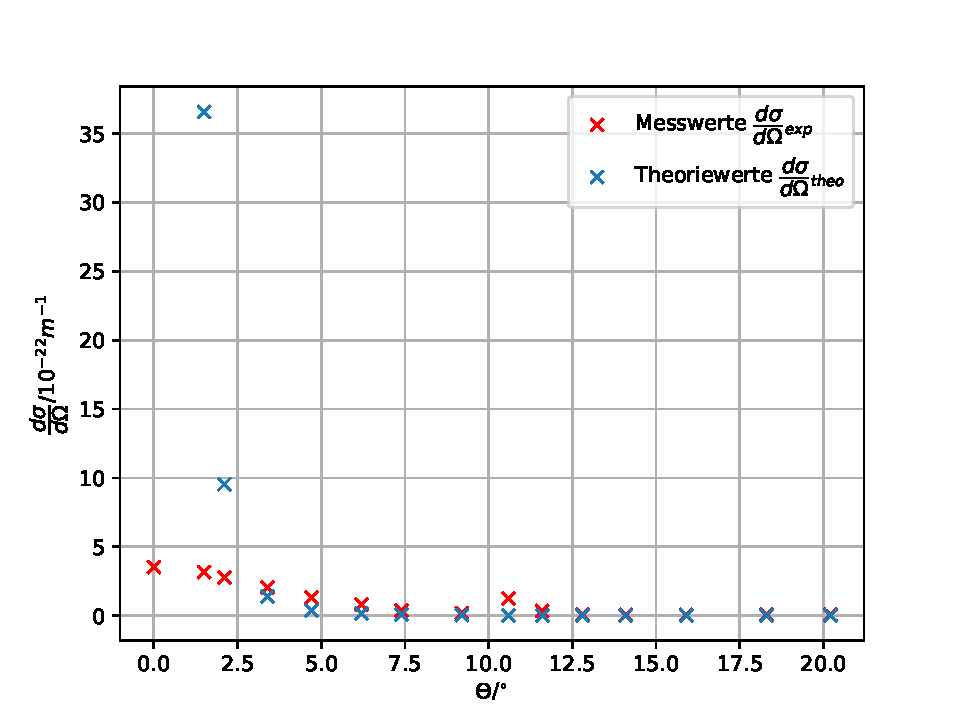
\includegraphics[height=8cm,width=12cm]{querschnitt.pdf}
	\caption{ Theoretischer und gemessener Wirkungsquerschnitt in Abhängigkeit des Streuwinkels}
	\label{fig: abb. 1}
	
	
\end{figure} 
\subsection{Mehrfachstreuung}
Bei einem festen Winkel von $\theta=15^{\circ}$ werden folgende Werte gemessen
\begin{table}[H] 
	\centering
	\begin{tabular}{c|c }
		
		Folienmaterial & n/t /s$^{-1}$ \\ 
		\hline 
		
		Gold (4  $\mu$m)& 0.22 $\pm$ 0,02  \\ 
		Gold (2 $\mu$m)& 0,10 $\pm$ 0,01
		
	\end{tabular} 
	\caption{Messwerte für verschiedene Foliendicken } 
\end{table} 
Dabei beträgt die Messzeit von Gold (4  $\mu$m) $t=$600 s und die Zählrate $n$=130.  Der Wert von Gold (2  $\mu$m) wurde über die Zählraten der Winkel $\theta_1=14,1^{\circ}$ und $\theta_2=15,9^{\circ}$ gemittelt. Für die zwei Goldfolien wurden folgende Streuquerschnitte berechnet:
\begin{align*}
\frac{d\sigma}{d\Omega} (\theta)_{4  \mu m}=(5,66 \cdot 10^{-24}) \text{m}^2\\
\frac{d\sigma}{d\Omega} (\theta)_{2  \mu m}=(5,14\cdot 10^{-24}) \text{m}^2\
\end{align*}

\subsection{Z-Abhängigkeit unterschiedlicher Folien}

Die Messwerte für die Folien aus verschiedenen Materialien sind in Tabelle 6 aufgelistet. Außerdem sind die zur Beschreibung der Z-Abhängigkeit benötigten Stoffeigenschaften$^{[5,6,7]}$ebenfalls in der Tabelle  zu finden. 

\begin{table}[H] 
	\centering
	\begin{tabular}{c|c c c c c c }
		
		Folienmaterial &Dichte $\rho / \frac{kg}{m^3}$& Z & A & N /$\cdot 10^{28} \frac{1}{m^3}$&  n/t /s$^{-1}$&$\dfrac{n/t}{Ndx} /\cdot10^{-24} m^2s^{-1}$ \\ 
		\hline 
		Aluminium (3 $\mu$m) &2.7 $\cdot 10^{4}$& 13 & 27& 6.022 & 0,68 $\pm$ 0,06 & 3,76 $\pm$ 0,04\\ 
		
		Bismut (1 $\mu$m)& 9.78 $\cdot 10^{4}$  & 83 & 209& 2.818 & 0,35 $\pm$ 0,05& 12,42 $\pm$ 1,32 \\ 
		
		Gold (2 $\mu$m) & 1.93   $\cdot 10^{4}$ & 79 & 197 & 5.910 &0,10 $\pm$ 0,03 & 0,85 $\pm$ 0,25  \\ 
		
	\end{tabular} 
	\caption{Messwerte für Folien aus unterschiedlichem Material} 
\end{table}
Um die Z-Abhängigkeit zu untersuchen, wird in Abbildung (7) $\frac{n/t}{N\cdot dx}$ gegen die Ordnungszahl Z aufgetragen: 
	\begin{figure}[H]
	
	\centering
	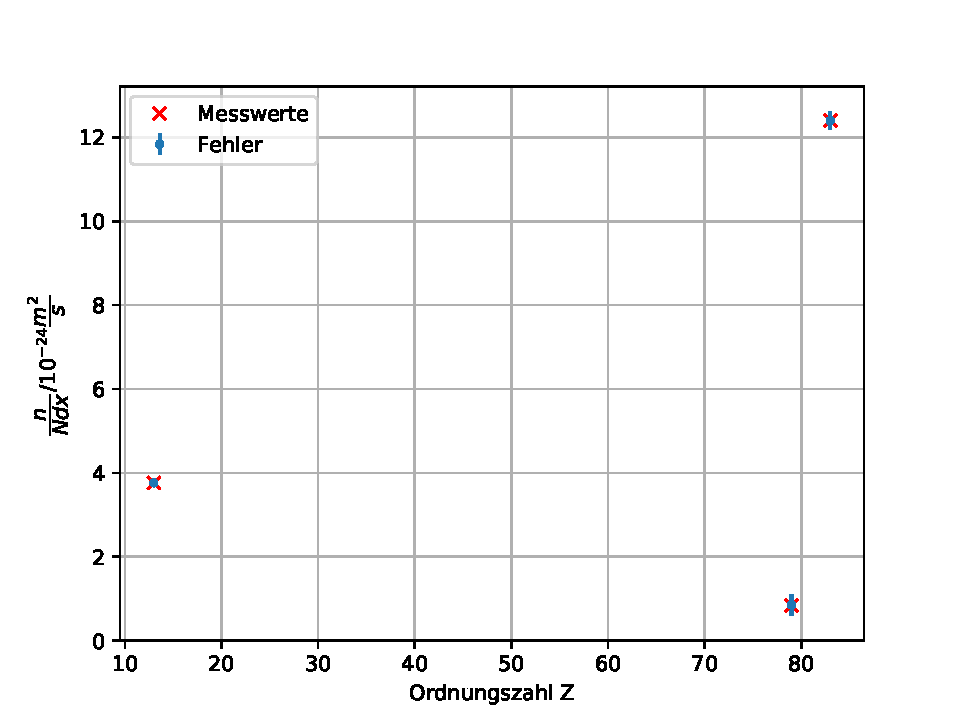
\includegraphics[height=8cm,width=12cm]{kernzahl.pdf}
	\caption{ Z-Abhängigkeit}
	\label{fig: abb. 1}
	
	
\end{figure} 

\section{Diskussion}
Beim Vergleich der zwei Pulse im Abschnitt 4.1 ist zunächst der unterschiedliche Verlauf zu erkennen. Beide entsprechen jedoch den Erwartungen. Weiterhin ist beim unverstärken Puls die Störungen deutlich zu sehen. Die Anstiegszeiten und die Pulshöhen wurden per Augenmaß abgelesen. Besonders bei dem unverstärkten Puls erwies sich die Bestimmung der Anstiegszeit als sehr schwierig aufgrund des senkrechten Anstiegs. \\\\
Bei der Bestimmung der Anfangsaktivität erhielten wir $A_{exp}=(21,52 \pm 0,31) \, \text{kBq}$. Der theoretische Wert beträgt $A_{theo}=317\, \text{kBq}$. Somit beträgt die Abweichung 92,1$\%$. Es zeigt sich, dass Radioaktivität und ionisierende Strahlung Zufallsprozesse sind und Vorhersagen schwierig zu treffen sind und dadurch Abweichungen bei Berechnungen auftreten können. \\\\
Bei der Bestimmung der Foliendicke in Abschnitt 4.4 war laut Herstellerangaben eine Foliendicke von 2 $\mu \text{m}$ zu erwarten. Der aus den Messwerten berechnete Wert $dx=(3,45\pm 0,13) \mu\text{m}$, weicht mit 42$\%$ vom Theoriewert ab. In der Abbildung 5 ist deutlich zu erkennen, dass die Pulshöhe nur sehr gering von der Ausgleichsgerade abweicht. Auch die zwei Steigungen weisen eine geringe Abweichung von 8$\%$ auf. Daraus wird deutlich, dass der Energieverlust durch Zufuhr der Luft proportional bei beiden Messungen zunimmt. Jedoch kann nicht erwartet werden, dass dieser exakt gleich ist, da die Energieabgabe der Alpha Teilchen an die Luftteilchen ein statistischer Prozess ist. Außerdem ist zu bemerken, dass  verschiedene Energieübergänge möglich sind, sodass die Annahme mit  $E_{\alpha}=5,27\cdot10^6 \text{eV}$ nicht der Realität entspricht. Die Bestrahlung mit monoenergetischen $\alpha$-Teilchen ist demnach nicht gewährleistet.\\\\
Auch in der Abbildung (6) ist zu erkennen, wie stark die berechneten Wirkungsquerschnitte von den theoretischen im Bereich von 0$^{\circ}$ bis 2,1 $^{\circ}$ abweichen. Jedoch nähern sich die Werte im weiteren Verlauf sehr stark an. Ab dem Winkel von 10,1$^{\circ}$ sieht man einen kleine Abweichung nach oben. An dieser Stelle wurde die Verstärkung verstellt.  Mögliche Gründe für die anfängliche Abweichungen sind unter anderem, dass die Wechselwirkungen mit den Hüllenelektronen bei der Rutherfordschen Streuformel vernachlässigt werden. Dadurch hat die Vernachlässigung des Energieverlust eine Abweichung des Messwertes zur Folge. Außerdem wurden einige Fehler in der Versuchsdurchführung gemacht. Während der Messreihe wurden unterschiedliche Verstärkungen durchgeführt, da der Counter bei größeren Winkel nur sehr wenig Pulse registrieren konnte. \\\\
Bei der Mehrfachstreuung lässt sich kein Vergleich der Messwerte machen, da die Zählrate $n/t$ bei Gold mit der Dicke von $2\, \mu$m unerwartet kleiner als bei der dickeren Folie ist. Dies könnte daran liegen, dass die Zählrate nicht gemessen, sondern aus zwei Messwerten gemittelt wurde, da wir keine Messung der dünneren Goldfolie bei genau 15 $^{\circ}$ durchgeführt haben. Weiterer Grund ist die schon oben erwähnte Verstellung des Verstärkers. \\\\
Auch im letzten Versuchsteil scheinen die Messwerte nicht ganz dem theoretischen Verlauf zu entsprechen. Die Messung konnte aufgrund fehlender Materialien nicht durchgeführt werden, sodass für Aluminium und Bismut mit theoretischen Werten gerechnet wurde. Lediglich der Wert von Gold ist aufgrund der vorherigen Versuchsdurchfühung stark fehlerbehaftet, was auch für den fehlerhaften Verlauf der Abbildung verantwortlich ist. Da der Wirkungsquerschnitt proportional zum Quadrat der Kernladungszahl ist, ist ein parabelförmiger Zusammenhang zu erwarten. 

\section{Literatur}
[1]: Versuchsprotokoll zum Versuch V16: Rutherford-Streuversuch \\ http://129.217.224.2/HOMEPAGE/PHYSIKER/BACHELOR/FP/SKRIPT/Rutherford.pdf 
\\ $[2]$ : Termschema
\\  http://archive.is/f8fyZ
\\ $[3]$ : Dichte von Luft \\
http://www.chemie.de/lexikon/Luftdichte.html\\
$[4]$: Eigenschaften Stickstoff und Sauerstoff \\
http://www.chemie.de/lexikon/Stickstoff.html\\
http://www.chemie.de/lexikon/Sauerstoff.html
\\ $[5]$ : Eigenschaften von Gold \\ http://www.chemie.de/lexikon/Gold.html
\\ $[6]$: Eigenschaften von Bismut \\ 
http://www.chemie.de/lexikon/Bismut.html 
\\ $[7]$ : Eigenschaften von Aluminium \\
http://www.chemie.de/lexikon/Aluminium.html  
\\ $[8]$: Ionisationsenergie von Gold \\
http://pdg.lbl.gov/2018/AtomicNuclearProperties/HTML/gold.Au.html\\
$[9]$: Differentieller Wirkungsquerschnitt\\
http://www.semibyte.de/wp/download/physics/versuchsprotokolle/f-praktikum-protokolle/311-rutherford-streuung.pdf\\


\end{document}